% !TeX program = pdflatex
% !BIB program = bibtex
\documentclass[journal]{IEEEtran}

\usepackage{iftex}
\ifPDFTeX
  \usepackage[T1]{fontenc}
  \usepackage[utf8]{inputenc}
\else
  \usepackage{fontspec}
  \setmainfont{TeX Gyre Termes}
  \setsansfont{TeX Gyre Heros}
  \setmonofont{TeX Gyre Cursor}
\fi
\usepackage{amsmath,amssymb}
\usepackage{graphicx}
\usepackage{booktabs}
\usepackage{tabularx}
\usepackage{multirow}
\usepackage{siunitx}
\usepackage{cite}
\usepackage{xurl}
\usepackage{tikz}
\usetikzlibrary{arrows.meta,positioning,fit,calc}
\usepackage{pgfplots}
\pgfplotsset{compat=1.18}
\usepackage[hidelinks]{hyperref}
\urlstyle{same}
\hypersetup{
  pdftitle={HARP-Net CKM: Prior Anchored Deep Learning for Dense UAV Channel Knowledge Maps},
  pdfauthor={Guillem Moreno Garcia, Evgenii Vinogradov, Sergi Abadal},
  pdfsubject={Dense UAV channel knowledge map prediction with frozen priors and bounded residual learning},
  pdfkeywords={channel knowledge map, UAV, 6G, channel attenuation, delay spread, angular spread, Gaussian mixture model}
}

\graphicspath{{./}}
\sisetup{detect-all=true}
\setlength{\textfloatsep}{6pt plus 1pt minus 2pt}
\setlength{\floatsep}{6pt plus 1pt minus 2pt}
\setlength{\intextsep}{6pt plus 1pt minus 2pt}
\setlength{\dbltextfloatsep}{6pt plus 1pt minus 2pt}
\setlength{\dblfloatsep}{6pt plus 1pt minus 2pt}

\title{\textsc{HARP-Net CKM}: Prior Anchored Deep Learning for Dense UAV Channel Knowledge Maps}

\author{Guillem Moreno Garcia, Evgenii Vinogradov, and Sergi Abadal%
\thanks{G. Moreno Garcia, E. Vinogradov, and S. Abadal are with the
Universitat Politecnica de Catalunya (UPC), Barcelona, Spain. Contact:
guillem.moreno.garcia@estudiantat.upc.edu.}%
}

\begin{document}
\bstctlcite{IEEEexample:BSTcontrol}
\maketitle

\begin{abstract}
Channel knowledge maps (CKMs) can turn expensive ray tracing into fast radio
planning, but dense UAV CKM generation remains difficult when channel
attenuation, delay spread, and angular spread must transfer to unseen cities.
This paper presents \textsc{HARP-Net CKM} (Height Aware Residual Prior Network
for Channel Knowledge Map prediction), a prior anchored surrogate. The method
first calibrates frozen physical and statistical priors on training cities
only: coherent two-ray and NLoS attenuation priors, plus log domain DS/AS
spread priors. A shared height conditioned residual network then predicts
bounded, distribution aware residuals instead of full maps from scratch. The
model receives a building height map, support/visibility masks, five frozen
prior maps, and scalar UAV transmitter height, and outputs three dense
\(513\times513\) maps. On a 14 city held out test split it reaches
\SI{1.6947}{dB} attenuation RMSE, \SI{26.6882}{ns} delay spread RMSE, and
\(11.5253^\circ\) angular spread RMSE, improving the frozen priors for all
three targets. The result supports a practical design rule: keep stable radial,
visibility, height, and spread structure in auditable priors, and spend neural
capacity on the residual structure that remains.
\end{abstract}

\begin{IEEEkeywords}
channel knowledge maps, UAV communications, radio map prediction, channel attenuation,
delay spread, angular spread, Gaussian mixture models, physics informed
learning.
\end{IEEEkeywords}

\section{Introduction and Related Work}

Channel knowledge maps (CKMs) store or predict radio channel quantities as
functions of position and environment, enabling faster planning and adaptation
than repeated ray tracing or exhaustive measurements \cite{zengx2021ckm,
ckmtutorial2024}. In UAV enabled 6G networks, CKMs are especially attractive
because altitude changes both the geometry and the line of sight probability of
the link \cite{khawaja_survey,saboor2025height}. A practical CKM surrogate,
however, must generalize to urban layouts not seen during training and must not
hide hard propagation regimes behind a single global score.

The central difficulty is that the three targets do not behave like one smooth
image regression problem. LoS attenuation has strong radial, height dependent
and two-ray structure; NLoS attenuation depends on blocked link regimes; and
delay and angular spread combine near zero LoS values with heavier NLoS tails.
Development experiments confirmed that a generic dense regressor can draw
plausible maps while still hiding NLoS mode collapse or poor spread tails.
The final design therefore separates the task into train only priors for stable
structure and a bounded neural residual for what remains.

The contribution is \textsc{HARP-Net CKM}, the Height Aware Residual Prior
Network for Channel Knowledge Map prediction. It is a dense CKM recipe for one
fixed UAV evaluation setting: strict city holdout, valid receiver masking,
explicit LoS/NLoS and height reporting, priors calibrated only on the training
split, and a neural residual model anchored to those priors. The paper also reports
city, height and visibility diagnostics so the final average is not presented
as a single opaque score.

\subsection{Radio Map and Channel Parameter Predictors}

Dense radio map prediction is often framed as image to image regression.
RadioUNet \cite{radiounet2020}, PMNet, and the ICASSP path loss challenge
family showed that U-Net style models can be strong dense channel attenuation baselines
\cite{pmnet2023,pmnet_icassp2023,icassp2023challenge}. Later work adds
attention, equivariance, domain shift handling, corridor weighting, or digital
twin generation \cite{rmtransformer2025,radiogunet2025,pathfinder2025,
gao2026,airmap2025}. These papers give the closest dense channel attenuation context, but not
the same setting: continuous UAV transmitter height, strict city holdout on CKM samples,
and three dense targets (channel attenuation/PL, DS, AS).

CKM work also emphasizes that a radio map is not merely an image but a
position indexed channel side information object \cite{zengx2021ckm,
ckmtutorial2024,ckmdata2024}. A random image split can place visually similar
urban layouts in both training and testing; a city split tests transfer to
unseen layouts, so the evaluation protocol is part of the method.

Physics informed and hybrid methods address a different weakness of pure image
regression: the model should not need to rediscover stable propagation effects
from pixels alone. ReVeal \cite{reveal2025} uses physics informed constraints
for radio environment mapping, while classical air to ground, COST/Hata, and
two-ray models encode known distance, height, reflection, and elevation angle
structure \cite{rappaport,goldsmith,cost231,alhourani2014,khawaja_survey,
tr38901,wocc2021}. This paper uses those models only as shape priors; all
deployment coefficients are calibrated from training cities under the same CKM
masking convention used at inference.

The spread side has fewer direct dense map references. Yang et al.\ predict
A2G delay spread with classical regressors \cite{yang2019a2gml}; Huang et al.\
use a Transformer style UAV mmWave predictor for received power, RMS delay
spread, and RMS angular spread \cite{huang2025a2gtransformer}; and Mi et al.\
predict mmWave channel attenuation (PL), DS, AS, and \(K\)-factor from measurement linked point
clouds \cite{mi2024pointcloud}. A closer map based reference is the multitask
super resolution model of Wang et al.\ \cite{wang2023multitasksr}, which
reconstructs path loss, delay spread, RMS azimuth/elevation angular spread and
LoS/NLoS maps from lower resolution channel maps. This is still a different
input contract: the low resolution channel field already contains sampled DS/AS
structure, whereas this paper generates dense \(513\times513\) CKM maps from
topology, support masks, priors and continuous UAV height for unseen cities.

Finally, heteroscedastic regression \cite{kendall2017uncertainties}, mixture
density wireless predictors \cite{saleh2021probabilistic,garciamarti2020mixture,
lee2024timevarying}, and stochastic radio map models \cite{radiodiff2025}
all point to the same issue: NLoS and spread targets are not well represented
by a single symmetric residual. For DS/AS, the closest external references are
therefore context rather than direct CKM benchmarks.

\section{Dataset and Evaluation Setting}

Each sample is a \(513\times513\) urban topology map from the ray traced CKM
setting used in this work. The carrier is fixed at
\SI{7.125}{GHz}, so frequency is not a learned variable; the main transmitter
degree of freedom is height. There is one UAV transmitter at the map centre.
The transmitter horizontal position is fixed, but its antenna height
\(h_{\mathrm{tx}}\) varies by sample and is treated as a central conditioning
variable rather than as metadata. The released CKM files call this node a UAV,
but the model setting is an elevated \SI{7.125}{GHz} transmitter within the
sampled height range, so the same setup can also represent other elevated radio
access nodes under the same simulation assumptions. The spatial resolution is
\SI{1}{m}\(\times\)\SI{1}{m} per pixel. Every non building pixel is treated as
an active receiver location, with the receiver antenna placed at
\(h_{\mathrm{rx}}=\SI{1.5}{m}\) above the ground. Building pixels are excluded
from the receiver set rather than treated as easy zero error targets. The model
predicts three aligned dense maps:
\[
  y_t \in \{\mathrm{PL~(dB)}, \mathrm{DS~(ns)}, \mathrm{AS~(deg)}\}.
\]
The CKM HDF5 field and implementation call the first target \texttt{path\_loss}
and retain the abbreviation PL. In this paper, PL is interpreted as the dense
channel attenuation map in dB, while \emph{path loss} is kept for standard
propagation formulas, cited path loss models, and dataset/code names that use
that term.
Let \(m_i(p)=1\) if pixel \(p\) of sample \(i\) is one of these valid ground
receivers, and zero otherwise. For a split \(\mathcal{S}\), the
target specific pixel weighted RMSE is
\begin{equation}
  \mathrm{RMSE}_t =
  \sqrt{
  \frac{\sum_{i\in\mathcal{S}}\sum_p m_i(p)
  \left(\hat{y}_{i,t}(p)-y_{i,t}(p)\right)^2}
  {\sum_{i\in\mathcal{S}}\sum_p m_i(p)}}.
  \label{eq:rmse}
\end{equation}
The same receiver-mask formula is used for all three targets. For DS and AS,
each valid ground pixel is still a receiver with a ray-traced ground truth
spread value, so the reported spread RMSE is the dense prediction compared with
the dense CKM target over all valid ground receivers.
To check whether the residual model improves spatial structure rather than only
global scale, this paper also reports map correlation:
\[
\begin{aligned}
\mathrm{MapCorr}_t
&=
\frac{\sum_{i\in\mathcal{C}_t} N_i\,\rho_{i,t}}
{\sum_{i\in\mathcal{C}_t} N_i},\\
\rho_{i,t}=
&\frac{\tilde{\hat{\mathbf y}}_{i,t}^{\top}\tilde{\mathbf y}_{i,t}}
{\|\tilde{\hat{\mathbf y}}_{i,t}\|_2\,\|\tilde{\mathbf y}_{i,t}\|_2}.
\end{aligned}
\]
where \(\Omega_i=\{p:m_i(p)=1\}\), \(N_i=|\Omega_i|\), and
\(\tilde{\mathbf y}_{i,t}\) and \(\tilde{\hat{\mathbf y}}_{i,t}\) are the valid
pixel vectors after subtracting their own per-map means. The set
\(\mathcal{C}_t\) excludes maps with fewer than two valid pixels or zero
variance in either vector. This is Pearson correlation after each map is centred
and normalized over its own valid receiver pixels, then averaged by valid pixel
count. Higher values mean that high and low regions are placed more similarly
to the ray traced target; RMSE remains the primary unit aware metric.

The split is city based rather than random over pixels or tiles. This matters:
random splits would allow the model to see nearly identical urban morphology
during training and testing. The final held out test split contains 2590
samples from cities not used to optimize model weights. Validation is used for
model selection; test is used only for the final generalization claim.
Table~\ref{tab:split-city-assignment} lists the exact city assignment.
Unless explicitly stated otherwise, every final model result reported below
refers to the separate 2590-sample, 14-city test split.

\begin{table}[!t]
\centering
\caption{Experimental setting used for all reported final numbers.}
\label{tab:experimental-setting}
\scriptsize
\setlength{\tabcolsep}{4pt}
\begin{tabularx}{\linewidth}{p{0.31\linewidth}X}
\toprule
Item & Setting \\
\midrule
Map resolution & \(513\times513\), \SI{1}{m}\(\times\)\SI{1}{m} pixels \\
Carrier / receiver & \SI{7.125}{GHz}; \(h_{\mathrm{rx}}=\SI{1.5}{m}\) \\
Transmitter & One centred UAV; stored \(h_{\mathrm{tx}}\approx\SIrange{12}{478}{m}\), nominal beta law \(\SIrange{10}{500}{m}\) \\
Inputs & Topology, ground/visibility masks, frozen priors, scalar height code \\
Targets & Channel attenuation / PL (dB), DS (ns), AS (deg), one dense map per target \\
Stored target ranges & PL \SIrange{65}{184}{dB}, DS \SIrange{0}{910}{ns}, AS \(0^\circ\)--\(180^\circ\) over all valid receivers \\
Metric mask & Non building ground receivers only; building pixels excluded \\
Split policy & City holdout; validation selects the checkpoint, test is final only \\
Samples & Train 10840; validation 2750; test 2590; all 16180 \\
\bottomrule
\end{tabularx}
\end{table}

\begin{table*}[!t]
\centering
\caption{City holdout assignment used by the distribution first and final neural models.}
\label{tab:split-city-assignment}
\scriptsize
\setlength{\tabcolsep}{4pt}
\begin{tabularx}{\textwidth}{lrrX}
\toprule
Split & Samples & Cities & City names \\
\midrule
Train & 10840 & 37 & Abidjan, Abu Dhabi, Alexandria, Antigua Guatemala,
Athens, Bangalore, Bangkok, Bath, Berlin, Bratislava, Brugge, Buenos Aires,
Canberra, Chefchaouen, Dalian, Hanoi, Ho Chi Minh City, Hyderabad, Kinshasa,
Leuven, Ljubljana, Luanda, Lyon, Manaus, Minsk, Nagpur, Paris,
Rio de Janeiro, Santiago, Shanghai, Siem Reap, St.~Louis, Thane, Toledo,
Valparaiso, Venice, Vienna. \\
Validation & 2750 & 15 & Bilbao, Chiang Mai, Cleveland, Dhaka, Dubrovnik,
Fortaleza, Marrakesh, Mexico City, Munich, Nazareth, Nice, Salvador, Segovia,
Tunis, Victoria. \\
Test & 2590 & 14 & Barcelona, Beijing, Carcassonne, Copenhagen, Halifax,
Jaipur, Johannesburg, Key West, Kuala Lumpur, Osaka, Phuket, Pune, Surat,
Vancouver. \\
\bottomrule
\end{tabularx}
\end{table*}

The transmitter height distribution is intentionally not uniform. Direct
comparison against the stored HDF5 histogram shows that the closest tested
affine version of the approximate double beta sampler is the original
\(h_{\mathrm{design}}\approx 10+490X\), with
\[
X\sim 0.75\,\mathrm{Beta}(3,23)+0.25\,\mathrm{Beta}(4,4),
\]
and nominal support \SIrange{10}{500}{m}. Reported results use the empirical
HDF5 realization: \(h_{\mathrm{tx}}\) spans \SIrange{11.61}{477.54}{m}, with
mean \SI{114.02}{m} and median \SI{75.66}{m}. Heights above \SI{478}{m} are
possible under the nominal law but rare, so the observed maximum is consistent
with finite sampling. Let \(\Delta h=\SI{3}{m}\),
\(B_k=[10+3k,\,13+3k)\), and \(h_i\) be the stored height of sample \(i\).
The reporting histogram is
\begin{equation}
  \begin{aligned}
  \hat f_{\Delta h}(h) &= d_k,\quad h\in B_k,\\
  d_k &= \frac{n_k}{N\Delta h},\quad
  n_k = \sum_{i=1}^{N}\mathbf{1}\{h_i\in B_k\},\quad N=16180 .
  \end{aligned}
  \label{eq:height-empirical-hist}
\end{equation}
For readability in Fig.~\ref{fig:height-density}, the plotted curve linearly
interpolates between the bin centre values \((c_k,d_k)\), with
\(c_k=11.5+3k\).
All database counts are 3972 samples below \SI{50}{m}, 8456 from
\SIrange{50}{150}{m}, 2490 from \SIrange{150}{300}{m}, and 1262 above
\SI{300}{m}; the corresponding training counts are 2676, 5654, 1644, and 866.
This skew also motivates the clipped logarithmic height feature used inside the
frozen priors: its denominator \(\log(401)\) corresponds to a practical
\SI{400}{m} transmitter to receiver height difference. The HDF5 maximum is
higher, but the higher altitude tail is thin after city and regime splitting,
so the normalization is chosen as a robust saturation scale rather than as the
absolute sample maximum.

\begin{figure}[!t]
\centering
\begin{tikzpicture}
\begin{axis}[
    width=0.97\linewidth,
    height=4.0cm,
    xlabel={Transmitter height \(h_{\mathrm{tx}}\) (m)},
    ylabel={Density (1/m)},
    xmin=0, xmax=500,
    ymin=0, ymax=0.014,
    xtick={0,50,150,300,500},
    scaled y ticks=false,
    yticklabel style={/pgf/number format/fixed, /pgf/number format/precision=3},
    axis lines=left,
    grid=major,
    tick label style={font=\scriptsize},
    label style={font=\scriptsize}
]
\addplot+[no marks, color=blue!70!black, thick]
table[x=mid_m,y=density,col sep=comma]{data/uav_height_histogram_3m.csv};
\end{axis}
\end{tikzpicture}
\caption{Empirical transmitter height density read directly from the CKM
HDF5 database using the \SI{3}{m} histogram of
\eqref{eq:height-empirical-hist}, linearly interpolated between bin centres
for display. Most training support lies in the low and middle altitude bands.}
\label{fig:height-density}
\end{figure}

\subsection{Quantized Targets and Continuous Outputs}

The released CKM targets are not ideal real valued measurements. Channel attenuation is
stored on an approximately \SI{1}{dB} grid, while delay spread and angular
spread are strongly integer valued and visibly staircase like in many maps. The
model outputs are not quantized to these grids: the residual network emits
continuous values, and all reported metrics compare those continuous outputs
against the stored targets. This matters for interpretation: the final path
loss MAE is \SI{0.9773}{dB}, close to the label step, while RMSE remains
\SI{1.6947}{dB} because it emphasizes hard tails. Less quantized labels would
likely expose more of the continuous surrogate's resolution, especially for
small residual improvements and spread map boundaries.

\section{\textsc{HARP-Net CKM} Framework}

\subsection{Why the Final Method Is Hybrid}

\textsc{HARP-Net CKM} separates stable structure from the residual structure
that remains hard to model analytically. First, the attenuation prior captures
LoS distance, height and two-ray effects and adds a calibrated NLoS branch for
blocked regions. Second, the spread priors use log domain regime calibration
for delay spread and angular spread. Third, the neural model receives these
frozen maps and predicts only bounded residual structure. This division keeps
the predictable part of the map auditable and reserves learning capacity for
the local errors that the frozen estimators cannot explain.

In this paper, a \emph{prior} means a frozen estimator fitted only on training
cities, not a hand tuned curve evaluated on the test set. The prior sees the
same support information available at deployment: centred transmitter geometry,
transmitter height, topology derived morphology, and a LoS/NLoS mask. In the
CKM benchmark runs, the stored HDF5 mask is used so every reported number uses
the same simulator support labels. For new datasets where only topology and
height are available, the generator ray casts the LoS/NLoS mask from those two
inputs; these generated masks are the operational support masks consumed by the
priors and by \textsc{HARP-Net CKM}. Once the prior coefficients and fallback
tables are stored, no gradient update is applied to them inside the neural
training loop. This separation is important because it lets the final residual
model be judged against a demanding baseline: the model must improve an already
calibrated predictor rather than merely beat FSPL.

The two lightweight regressors used inside the priors are standard least
squares tools. Ordinary least squares (OLS) fits linear coefficients by
minimizing training city squared error without regularization. Ridge regression
uses the same linear design matrix but adds an \(\ell_2\) penalty, which
stabilizes sparse height, topology, and visibility regimes.

\begin{figure*}[t]
\centering
\resizebox{0.96\textwidth}{!}{%
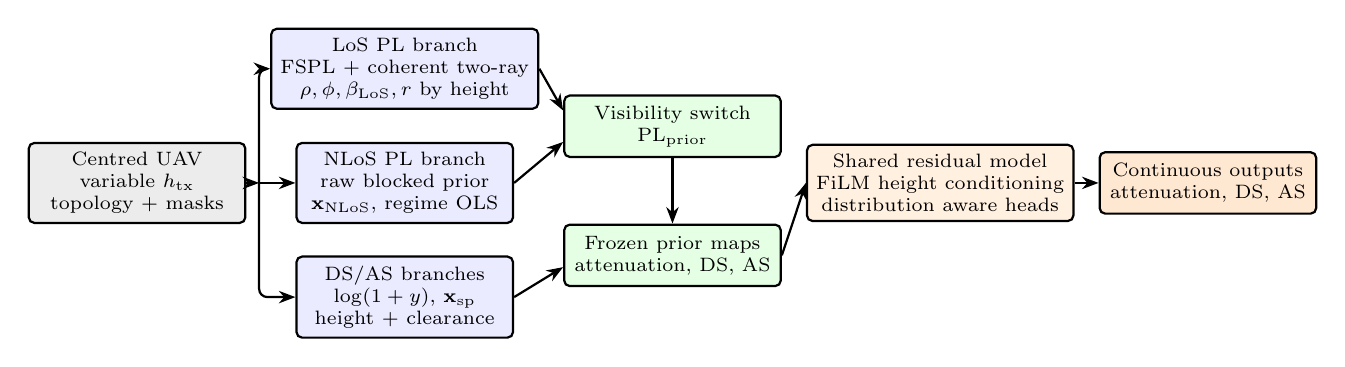
\begin{tikzpicture}[
  font=\scriptsize,
  box/.style={draw, thick, rounded corners=2pt, rectangle, minimum width=2.75cm, minimum height=0.78cm, align=center},
  input/.style={box, fill=gray!15},
  prior/.style={box, fill=blue!8},
  cal/.style={box, fill=green!10},
  model/.style={box, fill=orange!12},
  arr/.style={-{Stealth[length=2.1mm]}, thick, rounded corners=3pt}
]
\node[input] (support) at (0,0) {Centred UAV\\variable \(h_{\mathrm{tx}}\)\\topology + masks};
\node[prior] (los) at (3.4,1.45) {LoS PL branch\\FSPL + coherent two-ray\\\(\rho,\phi,\beta_{\mathrm{LoS}},r\) by height};
\node[prior] (nlos) at (3.4,0) {NLoS PL branch\\raw blocked prior\\\(\mathbf{x}_{\mathrm{NLoS}}\), regime OLS};
\node[prior] (spread) at (3.4,-1.45) {DS/AS branches\\\(\log(1+y)\), \(\mathbf{x}_{\mathrm{sp}}\)\\height + clearance};
\node[cal] (switch) at (6.8,0.72) {Visibility switch\\\(\mathrm{PL}_{\mathrm{prior}}\)};
\node[cal] (stack) at (6.8,-0.92) {Frozen prior maps\\attenuation, DS, AS};
\node[model] (net) at (10.2,0) {Shared residual model\\FiLM height conditioning\\distribution aware heads};
\node[input, fill=orange!18] (out) at (13.6,0) {Continuous outputs\\attenuation, DS, AS};

\coordinate (supportsplit) at (1.55,0);
\draw[arr] (support.east) -- (supportsplit);
\draw[arr] (supportsplit) |- (los.west);
\draw[arr] (supportsplit) -- (nlos.west);
\draw[arr] (supportsplit) |- (spread.west);
\draw[arr] (los.east) -- ([yshift=0.20cm]switch.west);
\draw[arr] (nlos.east) -- ([yshift=-0.20cm]switch.west);
\draw[arr] (switch.south) -- (stack.north);
\draw[arr] (spread.east) -- ([yshift=-0.15cm]stack.west);
\draw[arr] (stack.east) -- (net.west);
\draw[arr] (net.east) -- (out.west);
\end{tikzpicture}}
\caption{Compact \textsc{HARP-Net CKM} pipeline.
The transmitter is always centred, but its height varies by sample. Frozen
height aware priors are produced first and then used as channels for the final
\textsc{HARP-Net CKM} model.}
\label{fig:pipeline}
\end{figure*}

\begin{table}[!t]
\centering
\caption{Input/output definition of the full framework and final neural model.}
\label{tab:io-definition-paper}
\scriptsize
\setlength{\tabcolsep}{3pt}
\begin{tabularx}{\linewidth}{p{0.34\linewidth}X}
\toprule
Block & Variables \\
\midrule
External framework inputs &
Building height map and UAV transmitter height \(h_{\mathrm{tx}}\), stored as \texttt{uav\_height} in the CKM files. \\
Computed support maps &
LoS/NLoS visibility mask and valid ground receiver mask. \\
Frozen prior maps &
Combined path loss prior, LoS path loss prior, NLoS path loss prior,
delay spread prior, and angular spread prior. \\
Inputs to \textsc{HARP-Net CKM} &
Topology map, transmitter height conditioning, ground mask, LoS mask, NLoS mask,
and the five frozen prior maps. \\
Final outputs &
Channel attenuation, delay spread, and angular spread maps. \\
\bottomrule
\end{tabularx}
\end{table}

Thus the full generator has two external inputs and three final outputs. The
neural residual model has nine spatial map channels plus a separate scalar
transmitter height conditioning path because the framework has already computed
or loaded the visibility mask, receiver mask, and frozen prior maps.

\subsection{Frozen Priors}

The journal model is anchored by three deterministic maps fitted using
calibration-side cities disjoint from the final test environments: channel
attenuation, delay spread (DS), and angular spread (AS).
The attenuation construction is the subject of the companion conference
manuscript and is summarized here only to define the journal input contract.
% TODO: replace this sentence with the final conference citation after the
% conference manuscript receives a persistent identifier.

\subsubsection{Attenuation prior summary}
The attenuation prior separates visible and blocked links. For LoS pixels, the
starting structure is free-space loss plus a coherent direct/image-source
two-ray correction \cite{rappaport,goldsmith,wocc2021}. Effective reflection
amplitude and phase, a height-dependent bias, and a small radial residual table
are fitted in \SI{5}{m} transmitter-height bins, smoothed, and interpolated at
deployment. Operationally, these LoS correction terms form a height/radius
lookup table: it is frozen before testing and is not refitted in an unseen
city. For NLoS pixels, a conservative envelope of a COST231-shaped urban
trend and an elevation-dependent A2G term supplies the raw scale
\cite{cost231,alhourani2014,khawaja_survey}. A multiple linear (multilinear)
calibration then combines
that scale with range, elevation, local building density/height, and local NLoS
support. A geometric visibility mask selects the branches:
\begin{equation}
\begin{aligned}
\mathrm{PL}_{\mathrm{prior}}={}&m_{\mathrm{LoS}}
[\mathrm{FSPL}+C_{\mathrm{2ray}}+\beta_{\mathrm{LoS}}(h_{\mathrm{tx}})
+r(d_{2D},h_{\mathrm{tx}})]\\
&+(1-m_{\mathrm{LoS}})
\operatorname{clip}(\mathbf{x}_{\mathrm{NLoS}}^{\top}
\mathbf{w}_{\mathrm{NLoS},q},20,185).
\end{aligned}
\label{eq:concise-attenuation-prior}
\end{equation}
Here \(q\) denotes the supported morphology/height regime. The literature
provides formula shapes; the reflection curves, radial table, and NLoS weights
are CKM-specific training-split calibrations. This distinction prevents the
calibrated coefficients from being misread as transferable material constants.

\subsubsection{Spread priors}
DS and AS have a near-zero bulk and a long blocked-link tail. Their frozen
priors are therefore calibrated in the transformed domain
\begin{equation}
z=\log(1+y),\qquad \hat y=\exp(\hat z)-1,
\label{eq:spread-transform-paper}
\end{equation}
consistent with the log-domain treatment of large-scale spread parameters in
standard channel models \cite{tr38901,winner2}. A simple raw log prior uses
LoS/NLoS anchors, a topology offset, logarithmic range, inverse elevation,
local building density and height, and local NLoS support. The calibrated
feature vector augments this structure with transmitter height, blocker depth,
clearance, taller-building fraction, and selected interactions. For metric and
regime (q), ridge calibration gives
\begin{equation}
\widehat{\mathbf w}_{q}=
(\mathbf X^{\top}\mathbf X+\lambda\mathbf D^{\top}\mathbf D)^{-1}
\mathbf X^{\top}\mathbf z,\qquad
\hat z=\mathbf x_{\mathrm{sp}}^{\top}\widehat{\mathbf w}_{q}.
\label{eq:concise-spread-prior}
\end{equation}
The regularizer keeps the fitted map near the physically ordered raw prior
unless training residuals consistently support a change. Exact
topology/visibility/height keys fall back to compatible topology, visibility,
or global keys when support is insufficient. Thus rare high-spread pixels do
not determine an unsupported regime-specific curve.

All three priors are frozen before residual-network training. The neural model
receives the deployed maps rather than the handcrafted feature vectors, so the
prior calibration remains a separate and auditable preprocessing stage.
Table~\ref{tab:prior-only-anchor} reports the final test anchors.

\begin{table}[!t]
\centering
\caption{Frozen-prior RMSE on the final 14-city test split.}
\label{tab:prior-only-anchor}
\scriptsize
\setlength{\tabcolsep}{4pt}
\begin{tabular}{lrrrl}
\toprule
Target & Overall & LoS & NLoS & Unit \\
\midrule
Attenuation & 1.9383 & 1.7519 & 3.5143 & dB \\
Delay spread & 28.1211 & 27.5119 & 29.6157 & ns \\
Angular spread & 13.8162 & 15.3751 & 8.6614 & deg \\
\bottomrule
\end{tabular}
\end{table}

\subsection{HARP-Net CKM Residual Model}

The neural model receives nine aligned channels: topology, LoS mask, NLoS
mask, ground mask, combined path loss prior, LoS path loss prior, NLoS
path loss prior, delay spread prior, and angular spread prior. Height is
encoded with sinusoidal features and injected through FiLM modulation
\cite{perez2018film}, so the final network can adapt the residual field
continuously between the calibrated height regimes instead of learning one
height agnostic residual. The backbone is a shared U-Net style
encoder decoder with GroupNorm, FiLM conditioning, and task specific residual
heads.

The actual final model is therefore not a replacement for the priors. Its
input tensor already contains the deployed attenuation and spread estimates, and
its output head is constrained to learn bounded residuals around them. This
choice changes the learning problem: the encoder decoder does not need to infer
absolute free space attenuation, altitude trends, or the average spread scale
from pixels alone. It learns where the frozen estimates are locally biased and
how the remaining residual distribution should be placed across the map.

The height path mirrors the full implementation. The scalar
\(h_{\mathrm{tx}}\) is expanded to a 32-dimensional sinusoidal code using
16 log spaced frequencies over the transmitter height range,
\begin{equation}
\mathbf{e}(h_{\mathrm{tx}})
=
\left[
\sin\!\frac{h_{\mathrm{tx}}}{f_i},
\cos\!\frac{h_{\mathrm{tx}}}{f_i}
\right]_{i=1}^{16}
\in\mathbb{R}^{32},
\label{eq:height-embed-paper}
\end{equation}
then mapped by an MLP to a \(\mathbb{R}^{160}\) condition vector. Each FiLM
site projects this vector to channel wise scale and shift parameters and
modulates a feature map as
\begin{equation}
\mathbf{X}'=\mathbf{X}\odot(1+\mathbf{g})+\mathbf{b}.
\label{eq:film-paper}
\end{equation}
Encoder FiLM uses the height condition directly; decoder FiLM and the global
task heads use a fused condition formed from the height code and the pooled
bottleneck context. Thus the same centred topology can receive different
residual fields when the UAV is at \SI{30}{m}, \SI{150}{m}, or
\SI{350}{m}. The height aware results in Sec.~V show that this is not only an
architectural convenience: sinusoidal height embeddings with FiLM modulation are
sufficient for one model to cover the full varying height range without
training a separate network per altitude bin.

\begin{figure*}[!t]
\centering
\resizebox{0.98\textwidth}{!}{%
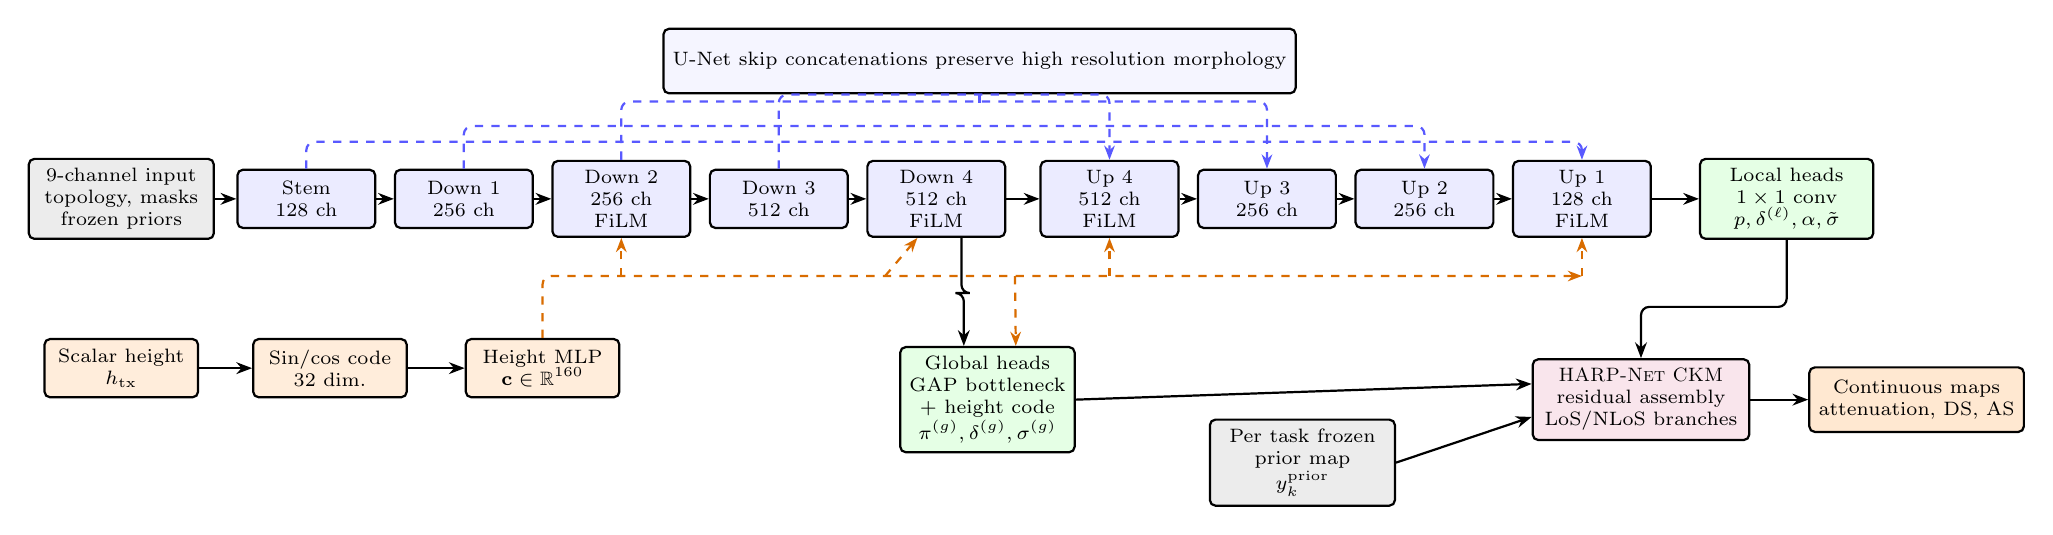
\begin{tikzpicture}[
  font=\scriptsize,
  block/.style={draw, thick, rounded corners=2pt, rectangle, minimum width=1.75cm, minimum height=0.74cm, align=center, fill=blue!8},
  cond/.style={draw, thick, rounded corners=2pt, rectangle, minimum width=1.95cm, minimum height=0.74cm, align=center, fill=orange!14},
  head/.style={draw, thick, rounded corners=2pt, rectangle, minimum width=2.2cm, minimum height=0.82cm, align=center, fill=green!10},
  gmm/.style={draw, thick, rounded corners=2pt, rectangle, minimum width=2.75cm, minimum height=1.0cm, align=center, fill=purple!10},
  prior/.style={draw, thick, rounded corners=2pt, rectangle, minimum width=2.35cm, minimum height=0.82cm, align=center, fill=gray!15},
  arr/.style={-{Stealth[length=2.0mm]}, thick, rounded corners=3pt},
  condarr/.style={-{Stealth[length=1.8mm]}, thick, dashed, orange!85!black, rounded corners=3pt},
  skiparr/.style={-{Stealth[length=1.8mm]}, thick, dashed, blue!65, rounded corners=3pt}
]
\node[prior] (input) at (0,0.8) {9-channel input\\topology, masks\\frozen priors};
\node[block] (stem) at (2.35,0.8) {Stem\\128 ch};
\node[block] (down1) at (4.35,0.8) {Down 1\\256 ch};
\node[block] (down2) at (6.35,0.8) {Down 2\\256 ch\\FiLM};
\node[block] (down3) at (8.35,0.8) {Down 3\\512 ch};
\node[block] (bott) at (10.35,0.8) {Down 4\\512 ch\\FiLM};
\node[block] (up4) at (12.55,0.8) {Up 4\\512 ch\\FiLM};
\node[block] (up3) at (14.55,0.8) {Up 3\\256 ch};
\node[block] (up2) at (16.55,0.8) {Up 2\\256 ch};
\node[block] (up1) at (18.55,0.8) {Up 1\\128 ch\\FiLM};
\node[head] (local) at (21.15,0.8) {Local heads\\\(1\times1\) conv\\\(p,\delta^{(\ell)},\alpha,\tilde\sigma\)};

\draw[arr] (input.east) -- (stem.west);
\draw[arr] (stem.east) -- (down1.west);
\draw[arr] (down1.east) -- (down2.west);
\draw[arr] (down2.east) -- (down3.west);
\draw[arr] (down3.east) -- (bott.west);
\draw[arr] (bott.east) -- (up4.west);
\draw[arr] (up4.east) -- (up3.west);
\draw[arr] (up3.east) -- (up2.west);
\draw[arr] (up2.east) -- (up1.west);
\draw[arr] (up1.east) -- (local.west);

\node[cond] (height) at (0,-1.35) {Scalar height\\\(h_{\mathrm{tx}}\)};
\node[cond] (embed) at (2.65,-1.35) {Sin/cos code\\32 dim.};
\node[cond] (hmlp) at (5.35,-1.35) {Height MLP\\\(\mathbf{c}\in\mathbb{R}^{160}\)};
\node[head] (global) at (11.0,-1.75) {Global heads\\GAP bottleneck\\+\ height code\\\(\pi^{(g)},\delta^{(g)},\sigma^{(g)}\)};
\node[prior] (taskprior) at (15.0,-2.55) {Per task frozen\\prior map\\\(y_k^{\mathrm{prior}}\)};
\node[gmm] (assembly) at (19.3,-1.75) {\textsc{HARP-Net CKM}\\residual assembly\\LoS/NLoS branches};
\node[prior, fill=orange!18] (out) at (22.8,-1.75) {Continuous maps\\attenuation, DS, AS};

\draw[arr] (height.east) -- (embed.west);
\draw[arr] (embed.east) -- (hmlp.west);
\coordinate (filmbusA) at (5.35,-0.18);
\coordinate (filmbusB) at (18.55,-0.18);
\draw[condarr] (hmlp.north) -- (filmbusA) -- (filmbusB);
\draw[condarr] (6.35,-0.18) -- (down2.south);
\draw[condarr] (9.70,-0.18) -- ([xshift=-0.24cm]bott.south);
\draw[condarr] (12.55,-0.18) -- (up4.south);
\draw[condarr] (18.55,-0.18) -- (up1.south);
\draw[condarr] (11.35,-0.18) -- ([xshift=0.36cm]global.north);

\draw[arr] ([xshift=0.32cm]bott.south) -- ++(0,-0.70) -| ([xshift=-0.30cm]global.north);
\draw[arr] (global.east) -- ([yshift=0.20cm]assembly.west);
\draw[arr] (local.south) -- ++(0,-0.85) -| (assembly.north);
\draw[arr] (taskprior.east) -- ([yshift=-0.22cm]assembly.west);
\draw[arr] (assembly.east) -- (out.west);

\node[prior, fill=blue!4, minimum width=5.2cm] (skip) at (10.9,2.55)
{U-Net skip concatenations preserve high resolution morphology};
\draw[skiparr] (stem.north) -- ++(0,0.34) -| (up1.north);
\draw[skiparr] (down1.north) -- ++(0,0.54) -| (up2.north);
\draw[skiparr] (down2.north) -- ++(0,0.74) -| (up3.north);
\draw[skiparr] (down3.north) -- ++(0,0.94) -| (up4.north);
\draw[blue!65, thick, dashed] (skip.south) -- ++(0,-0.18);
\end{tikzpicture}}
\caption{Final shared deep learning architecture used in the reported system
diagram. The map stack carries topology, masks, and frozen priors; the scalar
transmitter height is encoded separately and injected through FiLM. Encoder FiLM uses
the height code; decoder FiLM and global heads use the fused height/bottleneck
context. A shared U-Net produces local residual fields, pooled bottleneck
features produce global GMM parameters, and the \textsc{HARP-Net CKM} residual assembly
emits continuous channel attenuation, DS, and AS maps.
The blue dashed arrows show the four encoder--decoder concatenations used in
the implementation.}
\label{fig:dl-architecture}
\end{figure*}

The head uses a two branch residual logic around the frozen prior. The global branch asks:
``what residual distribution does this whole map, height, and topology imply?''
The local branch asks: ``where should each residual component be placed in the
\(513\times513\) map?'' This is the key distinction from a direct U-Net
regressor. The network does not directly overwrite the prior with a free form
map; it predicts a small residual distribution and then assigns that residual
pixel by pixel.

For each task \(k\), visibility region \(r\in\{\mathrm{LoS},\mathrm{NLoS}\}\),
component \(j\in\{1,2,3\}\), and pixel \(p\), the global head receives the
pooled bottleneck and fused height/context vector and outputs
\[
  \{\pi^{(g)}_{k,r,j},\delta^{(g)}_{k,r,j},\sigma^{(g)}_{k,r,j}\}_{j=1}^{3}.
\]
After the implementation transforms, \(\pi^{(g)}\) is a map level residual
mixture distribution, \(\delta^{(g)}\) is a bounded global residual offset, and
\(\sigma^{(g)}\) is a bounded global uncertainty scale. The local head receives
the full resolution decoder feature map and outputs
\[
  \{p_{k,r,j}(p)\}_{j=1}^{3},\quad
  \delta^{(\ell)}_{k,r}(p),\quad
  \alpha_{k,r}(p),\quad
  \tilde\sigma_{k,r}(p).
\]
Here \(p_{k,r,j}(p)\) is the per pixel component assignment, the local residual
\(\delta^{(\ell)}\) shifts all components at that pixel, \(\alpha\) is an
anchor gate initialized with bias \(-2\) so the model starts close to the
prior, and \(\tilde\sigma\) is the local uncertainty term. This extends the
distribution aware line of work from scalar mixture predictors to dense
residual maps \cite{saleh2021probabilistic,garciamarti2020mixture,
lee2024timevarying}. The native residual is clipped by target and visibility:
\begin{equation}
\Delta_{k,r,j}(p)
=\operatorname{clip}\!\left(
\delta^{(g)}_{k,r,j}+\delta^{(\ell)}_{k,r}(p),
-\delta_{\max,k,r},\delta_{\max,k,r}
\right),
\label{eq:delta-paper}
\end{equation}
with caps of \(7/25\) dB for attenuation (PL) LoS/NLoS, \(20/20\) ns for DS, and
\(17^\circ/15^\circ\) for AS. The residual cap is specified in native units:
dB for attenuation (PL), ns for DS, and degrees for AS. Omitting indices for compactness,
the component mean is anchored to the frozen prior after this native residual
has been assembled:
\begin{equation}
\begin{aligned}
u^{\mathrm{nat}}&=y^{\mathrm{prior,nat}}+\alpha\Delta,\\
\mu&=u^{\mathrm{nat}},\qquad k=\mathrm{PL},\\
\mu&=\log(1+[u^{\mathrm{nat}}]_+),\qquad k\in\{\mathrm{DS},\mathrm{AS}\}.
\end{aligned}
\label{eq:mu-paper}
\end{equation}
where \([u^{\mathrm{nat}}]_+=\max(u^{\mathrm{nat}},0)\) and
\(0\leq\alpha_{k,r}(p)\leq1\). The attenuation branch (PL) is modeled in native dB space, while DS and
AS use the log transform in \eqref{eq:spread-transform-paper}. The
deterministic map used for RMSE is the mixture mean in the modelled space:
\begin{equation}
\hat z_{k,r}(p)
=\sum_{j=1}^3p_{k,r,j}(p)\mu_{k,r,j}(p).
\label{eq:gmm-expectation-paper}
\end{equation}
For the attenuation branch (PL), \(\hat y_{k,r}=\hat z_{k,r}\). For DS and AS, the output is mapped
back with \(\hat y_{k,r}=\exp(\hat z_{k,r})-1\). Thus the spread output is
the deterministic point map used for RMSE, not the exact native space
expectation of the log space mixture.
The final map selects the LoS or NLoS branch with the explicit geometric mask.
The mixture variances combine map level and local uncertainty,
\begin{equation}
\sigma_{k,r,j}(p)
=
\sqrt{
\left(\sigma^{(g)}_{k,r,j}\right)^2
+
\left(\tilde\sigma_{k,r}(p)\right)^2
},
\label{eq:sigma-paper}
\end{equation}
with both terms constrained to \([0.05,3.0]\). During the probabilistic residual phase
these variances and mixture weights define a pixel wise likelihood; during the
final fine tuning phase the same head remains in place but the reported output
is the deterministic point map above.

The two mixture weight objects have different jobs. The global weights
\(\pi^{(g)}_{k,r,j}\) describe the sample level residual histogram and are
used by the distributional regularizer. The local weights \(p_{k,r,j}(p)\)
are the pixel wise assignment probabilities used in the final dense map. During
the probabilistic residual phase the per pixel density is
\begin{equation}
q_{k,r}(z_k(p)\mid p)
=
\sum_{j=1}^{3}
p_{k,r,j}(p)\,
\mathcal{N}\!\left(
z_k(p);\mu_{k,r,j}(p),\sigma^2_{k,r,j}(p)
\right),
\label{eq:gmm-density-paper}
\end{equation}
and the regional NLL is the masked average of
\(-\log q_{k,r}(z_k(p)\mid p)\) over valid LoS or NLoS pixels. Separately,
the KL term bins the true residuals
\(\epsilon_k(p)=y_k(p)-y^{\mathrm{prior}}_k(p)\) into a soft empirical
histogram and compares it with the histogram implied by
\(\{\pi^{(g)}_{k,r,j},\delta^{(g)}_{k,r,j}\}\). This is what makes the head
``distribution first'': before the decoder places values pixel by pixel, the
global branch is pressured to put mixture mass where the map residuals actually
live.

This head is useful even when the final reported number is a deterministic
RMSE. The probabilistic phase teaches the network that a hard NLoS region can
contain several plausible residual levels, while the anchor gate decides how
far the prediction may move from the frozen estimate. The final point map is
therefore not an unconstrained average of arbitrary map values; it is the
model space mean of a small residual mixture whose components remain tied to
the prior.

\begin{figure*}[!t]
\centering
\resizebox{0.96\textwidth}{!}{%
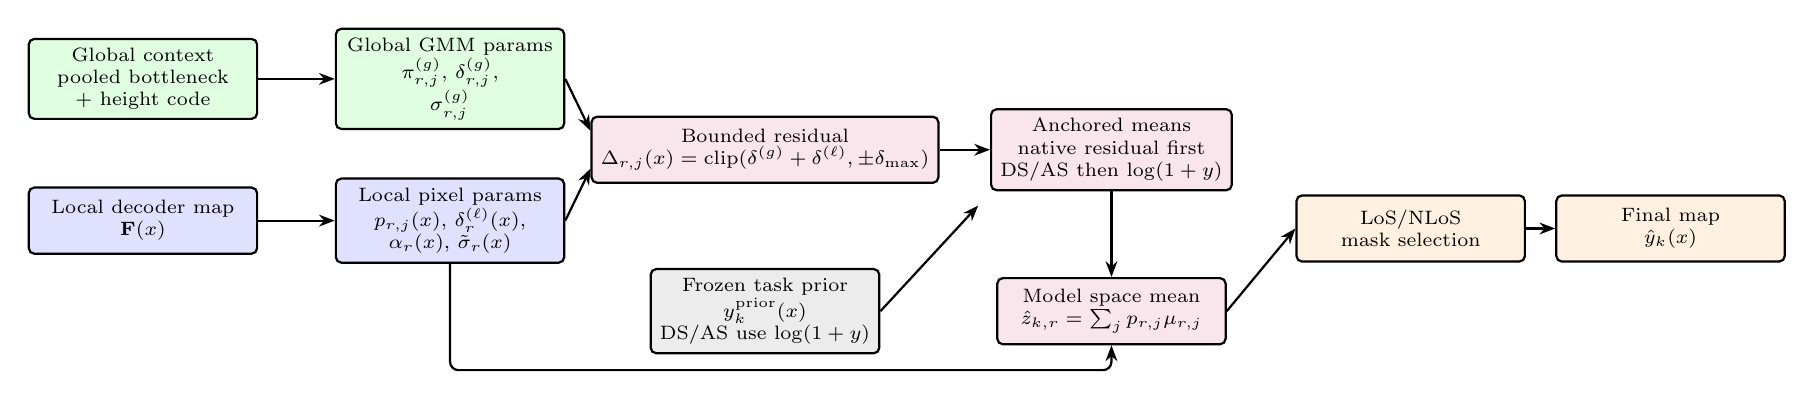
\begin{tikzpicture}[
  font=\scriptsize,
  box/.style={draw, thick, rounded corners=2pt, rectangle, minimum width=2.9cm, minimum height=0.84cm, align=center},
  global/.style={box, fill=green!12},
  local/.style={box, fill=blue!12},
  prior/.style={box, fill=gray!15},
  mix/.style={box, fill=purple!10},
  outbox/.style={box, fill=orange!12},
  arr/.style={-{Stealth[length=2.0mm]}, thick, rounded corners=3pt}
]
\node[global] (g0) at (0,1.6) {Global context\\pooled bottleneck\\+\ height code};
\node[global] (g1) at (3.9,1.6) {Global GMM params\\\(\pi^{(g)}_{r,j}\), \(\delta^{(g)}_{r,j}\),\\\(\sigma^{(g)}_{r,j}\)};
\node[local] (l0) at (0,-0.2) {Local decoder map\\\(\mathbf{F}(x)\)};
\node[local] (l1) at (3.9,-0.2) {Local pixel params\\\(p_{r,j}(x)\), \(\delta^{(\ell)}_r(x)\),\\\(\alpha_r(x)\), \(\tilde\sigma_r(x)\)};
\node[mix] (resid) at (7.9,0.7) {Bounded residual\\\(\Delta_{r,j}(x)=\mathrm{clip}(\delta^{(g)}+\delta^{(\ell)},\pm\delta_{\max})\)};
\node[prior] (p0) at (7.9,-1.35) {Frozen task prior\\\(y^{\mathrm{prior}}_k(x)\)\\DS/AS use \(\log(1+y)\)};
\node[mix] (mu) at (12.3,0.7) {Anchored means\\native residual first\\DS/AS then \(\log(1+y)\)};
\node[mix] (expv) at (12.3,-1.35) {Model space mean\\\(\hat z_{k,r}=\sum_j p_{r,j}\mu_{r,j}\)};
\node[outbox] (sel) at (16.1,-0.3) {LoS/NLoS\\mask selection};
\node[outbox] (out) at (19.4,-0.3) {Final map\\\(\hat y_k(x)\)};

\draw[arr] (g0.east) -- (g1.west);
\draw[arr] (l0.east) -- (l1.west);
\draw[arr] (g1.east) -- ([yshift=0.24cm]resid.west);
\draw[arr] (l1.east) -- ([yshift=-0.24cm]resid.west);
\draw[arr] (resid.east) -- (mu.west);
\draw[arr] (p0.east) -- ([xshift=-0.15cm,yshift=-0.18cm]mu.south west);
\draw[arr] (mu.south) -- (expv.north);
\draw[arr] (l1.south) -- ++(0,-1.35) -| (expv.south);
\draw[arr] (expv.east) -- (sel.west);
\draw[arr] (sel.east) -- (out.west);
\end{tikzpicture}}
\caption{\textsc{HARP-Net CKM} residual head. The global branch predicts the
sample level residual mixture; the local branch places that distribution
pixel by pixel through component weights, residual refinements, gates and local
uncertainty. Component means are anchored to the frozen prior and the
deterministic map is obtained from the pixel wise model space mixture mean after LoS/NLoS
selection.}
\label{fig:residual-head}
\end{figure*}

\textsc{HARP-Net CKM} should not be read as only the final fine tuning loss. It has two active
training phases: a large capacity probabilistic residual phase with probabilistic losses
enabled, followed by an RMSE/MAE dominant fine tuning phase. The composite
objective implemented by the model is
\begin{equation}
\begin{aligned}
\mathcal{L}
={}&
\sum_k w_k\bigl(
\lambda_{\mathrm{NLL}}\mathcal{L}_{\mathrm{NLL},k}
+\lambda_{\mathrm{KL}}\mathcal{L}_{\mathrm{KL},k}
+\lambda_{\mathrm{mom}}\mathcal{L}_{\mathrm{mom},k}\\
&+\lambda_{\mathrm{anchor}}\mathcal{L}_{\mathrm{anchor},k}
+\lambda_{\mathrm{guard}}\mathcal{L}_{\mathrm{guard},k}
+\lambda_{\mathrm{out}}\mathcal{L}_{\mathrm{out},k}\\
&+\lambda_{\mathrm{RMSE}}\mathcal{L}_{\mathrm{RMSE},k}
+\lambda_{\mathrm{MAE}}\mathcal{L}_{\mathrm{MAE},k}
\bigr).
\end{aligned}
\label{eq:loss}
\end{equation}

The probabilistic terms matter during the probabilistic residual phase. The NLL term
teaches the head to place mixture mass around the transformed target, the KL
and moment terms keep the mixture distribution from becoming a numerically
convenient but physically uninformative density, and the outlier budget term
discourages a solution that spends most of its capacity on the easy bulk while
leaving large tails unconstrained. The final fine tuning phase then disables
those terms and optimizes the deterministic mixture mean point map for RMSE/MAE,
with a small anchor and guard that keep the residual anchored to the prior.
Table~\ref{tab:loss-roles} summarizes the roles. The selected checkpoint is
therefore reported as a deterministic RMSE improvement over the frozen priors,
not as a calibrated probabilistic predictor. In this final phase, checkpoint
selection uses the validation composite
\(\mathrm{PL}_{\mathrm{RMSE}}+0.30\,\mathrm{DS}_{\mathrm{RMSE}}
+0.25\,\mathrm{AS}_{\mathrm{RMSE}}\), matching the reported
\texttt{score\_weights}.

\begin{table*}[!t]
\centering
\caption{Loss terms available in the \textsc{HARP-Net CKM} objective and their practical
purpose.}
\label{tab:loss-roles}
\scriptsize
\begin{tabularx}{\textwidth}{p{0.15\textwidth}p{0.18\textwidth}X}
\toprule
Term & Active phase & Role \\
\midrule
GMM NLL & probabilistic residual phase &
Fits the per pixel mixture density in native attenuation (PL) space and log transformed
spread space. \\
Distribution KL & probabilistic residual phase &
Regularizes the learned mixture so it remains close to the intended
distributional structure instead of using degenerate weights or variances. \\
Moment matching & probabilistic residual phase &
Encourages the model space mean and spread of the mixture to agree with target
moments, stabilizing deterministic extraction from the GMM. \\
Outlier budget & probabilistic residual phase &
Keeps rare large residuals visible in the objective instead of letting the
global average hide them. \\
Anchor & both phases &
Penalizes unnecessary deviation from the frozen prior; this is especially
important because the prior is already a strong calibrated predictor. \\
Prior guard & both phases &
Adds a penalty when the model becomes worse than the prior at valid pixels,
discouraging destructive residual shifts. \\
RMSE / MAE & both phases, dominant in final fine tuning &
Optimizes the deterministic map reported in the final evaluation; RMSE handles
tails and MAE tracks typical absolute error. \\
\bottomrule
\end{tabularx}
\end{table*}

\begin{table}[t]
\centering
\caption{Training configuration of the final line.}
\label{tab:training}
\scriptsize
\begin{tabularx}{\linewidth}{lX}
\toprule
Item & Value \\
\midrule
Image size & \(513\times513\) \\
Input channels & 9 map channels plus height FiLM conditioning \\
Backbone & GroupNorm U-Net, base width 128, FiLM dim. 160 \\
Residual head & 3 mixture components, bounded residuals \\
Optimizer & AdamW, learning rate \(5\times10^{-5}\), weight decay 0.01 \\
Batching & batch size 1, gradient accumulation 8 \\
Scheduler & 1 warmup epoch plus cosine \texttt{LambdaLR}; early stopping patience 10 \\
Augmentation & Training D4 rotations/reflections only; evaluation uses no augmentation \\
Checkpoint selection & Validation composite PL RMSE \(+0.30\) DS RMSE \(+0.25\) AS RMSE \\
Loss schedule & Large capacity probabilistic residual phase plus final residual
fine tuning; see Table~\ref{tab:loss-schedule} \\
\bottomrule
\end{tabularx}
\end{table}

\begin{table}[t]
\centering
\caption{\textsc{HARP-Net CKM} loss schedule. The pre fine tuning probabilistic residual phase is part
of the final pipeline, even though the reported checkpoint is selected after
the deterministic fine tuning phase.}
\label{tab:loss-schedule}
\scriptsize
\begin{tabularx}{\linewidth}{lXX}
\toprule
Setting & Probabilistic residual phase & Final fine tuning \\
\midrule
NLL / KL / moment / outlier & 1.00 / 0.25 / 0.10 / 0.02 & 0 / 0 / 0 / 0 \\
RMSE / MAE & 1.50 / 0.10 & 1.00 / 0.05 \\
Anchor / guard & 0.05 / 0.10 & 0.01 / 0.02 \\
Task weights & PL 1.0, DS 1.0, AS 1.0 & PL 1.0, DS 0.25, AS 0.25 \\
Learning rate & \(2\times10^{-4}\) & \(5\times10^{-5}\) \\
\bottomrule
\end{tabularx}
\end{table}

The practical role of the two training phases is simple. The first phase makes the head
behave like a residual density model: it learns where residual mass lies and
discourages the old single mode collapse. The final fine tuning phase keeps the
same architecture but shifts the optimization weight toward the deterministic
metrics used for the paper tables. The anchor and guard terms remain active at
small weight so the fine tuned model cannot gain average RMSE by damaging large
regions where the frozen prior was already accurate.

\section{Experiments and Results}

\subsection{Main Test Results and City Audit}

Before collapsing the test split to one average, Table~\ref{tab:test-city-audit}
shows the city level audit. Training cities are omitted because the priors and
the residual model were fitted on them; validation cities are used for model
selection and are not part of the final claim. The test rows show that the
aggregate result is not a single easy city effect. Osaka, Kuala Lumpur, Phuket,
Barcelona, and Pune are harder for delay spread, while Carcassonne, Halifax,
Key West, and Vancouver are easier under this split. The topology and height
mix columns explain part of this variation: cities with more low or mid height
samples and denser morphology generally show larger spread errors.

\begin{table*}[!t]
\centering
\caption{Held out test RMSE by city. Attenuation is in dB, delay spread in ns
and angular spread in degrees. Topology mix is open/mixed/dense; height mix is
low/mid/high antenna percentage.}
\label{tab:test-city-audit}
\scriptsize
\setlength{\tabcolsep}{3pt}
\begin{tabularx}{\textwidth}{>{\raggedright\arraybackslash}Xrrrrcc}
\toprule
City & Samples & Atten. & DS & AS & Topology mix & Height mix \\
\midrule
Barcelona & 50 & 1.74 & 33.0 & 11.1 & 30/30/40 & 40/32/28 \\
Beijing & 200 & 1.57 & 23.3 & 10.7 & 28/65/8 & 30/41/30 \\
Carcassonne & 110 & 1.43 & 8.0 & 9.7 & 41/50/9 & 30/29/41 \\
Copenhagen & 220 & 1.83 & 27.3 & 12.0 & 14/68/18 & 37/27/36 \\
Halifax & 250 & 1.43 & 19.9 & 9.7 & 78/22/0 & 36/33/31 \\
Jaipur & 120 & 2.05 & 21.6 & 11.9 & 12/25/62 & 37/34/29 \\
Johannesburg & 245 & 1.76 & 21.0 & 12.1 & 10/55/35 & 34/34/32 \\
Key West & 105 & 1.39 & 20.0 & 10.4 & 52/43/5 & 33/30/37 \\
Kuala Lumpur & 360 & 2.05 & 44.2 & 13.5 & 18/44/38 & 29/38/34 \\
Osaka & 50 & 2.43 & 37.3 & 14.9 & 0/60/40 & 28/44/28 \\
Phuket & 50 & 1.82 & 37.2 & 13.8 & 20/50/30 & 28/36/36 \\
Pune & 135 & 1.95 & 33.3 & 13.2 & 15/67/19 & 32/27/41 \\
Surat & 190 & 1.63 & 23.5 & 10.3 & 34/16/50 & 36/32/32 \\
Vancouver & 505 & 1.53 & 17.7 & 10.8 & 29/67/4 & 31/35/34 \\
\bottomrule
\end{tabularx}
\end{table*}

Table~\ref{tab:main-results} then collapses the same held out test split to the
target averages. The model reduces RMSE relative to the frozen prior for all
three targets. Channel attenuation is the cleanest success case because both
RMSE and MAE improve. Angular spread also improves strongly in RMSE and remains
approximately neutral in MAE. Delay spread improves RMSE while MAE slightly
increases; this is consistent with reducing rare high delay errors while
introducing small local shifts.

\begin{table*}[!t]
\centering
\caption{Final model test results on unseen cities. Negative \(\Delta\) means
that the residual model improves the frozen prior.}
\label{tab:main-results}
\scriptsize
\setlength{\tabcolsep}{4pt}
\begin{tabular}{lrrrrl}
\toprule
Target & Model RMSE & Prior RMSE & \(\Delta\)RMSE & Model MAE & Unit \\
\midrule
Attenuation & 1.6947 & 1.9383 & -0.2436 & 0.9772 & dB \\
Delay spread & 26.6882 & 28.1211 & -1.4329 & 7.8160 & ns \\
Angular spread & 11.5253 & 13.8162 & -2.2909 & 4.8899 & deg \\
\bottomrule
\end{tabular}
\end{table*}

\begin{table}[!t]
\centering
\caption{Final model test map correlation on unseen cities. Higher is better.}
\label{tab:mapcorr}
\scriptsize
\setlength{\tabcolsep}{4pt}
\begin{tabular}{lrrr}
\toprule
Target & Model & Prior & \(\Delta\) \\
\midrule
Attenuation & 0.961055 & 0.947710 & +0.013345 \\
Delay spread & 0.414692 & 0.306026 & +0.108666 \\
Angular spread & 0.581783 & 0.348713 & +0.233070 \\
\bottomrule
\end{tabular}
\end{table}

The original numerical targets were \SI{5}{dB}, \SI{50}{ns}, and
\(20^\circ\). The final model clears all three on unseen cities. More
importantly, it does so jointly: the same network predicts channel attenuation,
DS, and AS instead of
using separate specialist models.
The targets are broad acceptance thresholds rather than equally informative
final benchmarks. In particular, the attenuation prior is already below
\SI{2}{dB}, so the final attenuation question is whether the residual network
beats that prior and preserves map structure; Tables~\ref{tab:main-results}
and~\ref{tab:mapcorr} show that it does.
The map correlation results in Table~\ref{tab:mapcorr} add a structural check:
after each map's mean and scale are removed, the residual model places the
relative high and low regions better than the frozen priors for all three
targets. This is especially important for the spread maps. Delay spread RMSE
improves by about \(5\%\) and angular spread RMSE by about \(17\%\), but their
MapCorr values rise by about \(36\%\) and \(67\%\) relative to the frozen priors.
Thus the residual model is doing visible map structure recovery even when the
unit aware RMSE gain looks modest.

\paragraph{Channel attenuation}
The frozen path loss prior is already strong, reaching \SI{1.9383}{dB} RMSE
and \SI{1.2319}{dB} MAE on the final test split. \textsc{HARP-Net CKM}
reduces these to \SI{1.6947}{dB} and \SI{0.9772}{dB}. This is the most
uniform gain: the residual model improves both squared error and typical
absolute error, and it improves both LoS and NLoS pixels in
Table~\ref{tab:los-nlos}. The closest external references are dense path loss
radio map papers, but they still differ in split, height protocol, frequency,
and target definition.

\paragraph{Angular spread}
The angular spread prior reaches \(13.8162^\circ\) RMSE and \(5.0033^\circ\)
MAE; the final model reaches \(11.5253^\circ\) RMSE and \(4.8899^\circ\) MAE.
The MAE gain is smaller than the RMSE gain, so the residual model mainly suppresses larger angular
spread errors rather than shifting every pixel uniformly. The LoS gain is much
larger than the NLoS gain, which is expected because the NLoS angular spread
prior is already close to the target distribution. No reviewed external method
reports the same dense CKM city holdout angular spread map task. The nearest
papers either predict link level or sparse angular spread channel parameters
\cite{huang2025a2gtransformer,mi2024pointcloud}, or reconstruct channel
characteristic maps from lower resolution channel maps
\cite{wang2023multitasksr}. The primary numerical comparison is therefore
against the frozen prior and the same protocol target.

\paragraph{Delay spread}
The delay spread prior reaches \SI{28.1211}{ns} RMSE and \SI{7.3041}{ns} MAE;
the final model reaches \SI{26.6882}{ns} RMSE and \SI{7.8160}{ns} MAE. This
is the least uniform target: RMSE improves because rare high delay errors are
reduced, while MAE slightly worsens because small local shifts appear in many
easy pixels. The LoS/NLoS split confirms that the model improves both
visibility cases in RMSE. Similar A2G delay spread predictors exist
\cite{yang2019a2gml,huang2025a2gtransformer}, and Wang et al.\ provide a
map based super resolution reference \cite{wang2023multitasksr}. None is the
same topology to dense CKM city holdout generation task, so they are used as
context rather than as direct leaderboards.

\subsection{LoS/NLoS and Split Diagnostics}

Table~\ref{tab:los-nlos} separates valid pixels by the geometric visibility
mask. The residual model improves the prior in both LoS and NLoS pixels for all
targets. This is important because global RMSE could otherwise hide a failure
in the physically hard NLoS subset.

\begin{table}[t]
\centering
\caption{Final test RMSE separated by LoS and NLoS pixels.}
\label{tab:los-nlos}
\scriptsize
\begin{tabular}{llrrr}
\toprule
Target & Scope & Model & Prior & \(\Delta\) \\
\midrule
Atten. & LoS & 1.5175 & 1.7519 & -0.2344 \\
Atten. & NLoS & 3.1596 & 3.5143 & -0.3547 \\
DS & LoS & 25.6137 & 27.5119 & -1.8983 \\
DS & NLoS & 29.2464 & 29.6157 & -0.3693 \\
AS & LoS & 12.5270 & 15.3751 & -2.8481 \\
AS & NLoS & 8.4550 & 8.6614 & -0.2064 \\
\bottomrule
\end{tabular}
\end{table}

The validation/test sanity check is also useful. The validation row evaluates
the selected checkpoint on validation cities, while the test row is the real
generalization result. Delay spread worsens more on test because the
held out city mix contains harder high delay cases. The frozen delay spread
prior shows the same validation to test worsening, confirming that this is a
city mix effect rather than an evaluator change.

\begin{table}[t]
\centering
\caption{Validation versus held out test check for the same selected model.}
\label{tab:val-test}
\scriptsize
\begin{tabular}{lrrrr}
\toprule
Split & Samples & Atten. RMSE & DS RMSE & AS RMSE \\
\midrule
Validation & 2750 & 1.6272 & 22.1946 & 11.4141 \\
Test & 2590 & 1.6947 & 26.6882 & 11.5253 \\
\bottomrule
\end{tabular}
\end{table}

\begin{table*}[!t]
\centering
\caption{Held out test RMSE by antenna height bin. Each \(\Delta\) column is
model minus frozen prior, so negative is better.}
\label{tab:antenna-breakdown}
\scriptsize
\setlength{\tabcolsep}{4pt}
\begin{tabular}{lrrrrrrr}
\toprule
Antenna bin & Samples & PL & \(\Delta\)PL & DS & \(\Delta\)DS & AS & \(\Delta\)AS \\
\midrule
low & 846 & 1.8755 & -0.2645 & 35.33 & -2.02 & 13.15 & -2.36 \\
mid & 878 & 1.7382 & -0.2527 & 27.70 & -1.40 & 11.92 & -2.54 \\
high & 866 & 1.4990 & -0.2165 & 11.78 & -0.46 & 8.81 & -2.08 \\
\bottomrule
\end{tabular}
\end{table*}

The antenna breakdown in Table~\ref{tab:antenna-breakdown} is a held out test
audit, not a training result. It shows that all three height bins improve for
all targets. Low altitude remains the hardest spread regime, while high altitude
is easier for DS and AS because fewer rays are trapped by local rooftops and
street canyons.

\subsection{Prior and Split Breakdowns}

The frozen priors are strong enough to deserve their own reporting. They are
not simply baselines for the final neural model; they encode most of the stable
geometry and therefore determine what residual problem the network sees.
Because these prior calibrations are deterministic, non DL estimators, their
standalone audits are reported separately from neural checkpoint selection. The
path loss table uses the held out validation+test split after fitting the
10840 training references and evaluating 5340 held out references
(4994 topology assigned rows). The spread table uses the final 14-city test
split because the calibrated spread prior code and the final residual model use
the same 10840/2750/2590 train/validation/test split.
Table~\ref{tab:pl-prior-height} shows the height dependence of the calibrated
path loss prior. This is not post hoc stratification: transmitter height is part of the
prior estimator through the centred geometry, elevation angle, and
height binned calibration, and it later conditions the residual neural model
through FiLM. The trend is strongest in NLoS: the low altitude bin remains the
hardest because many receivers are blocked by local urban structure, while high
UAVs see fewer deep shadow pockets.
Table~\ref{tab:spread-prior-height} shows the matching spread prior pattern.
Delay spread in particular collapses with altitude, from \SI{39.90}{ns}
overall in the lowest bin to \SI{3.70}{ns} above \SI{300}{m}.
Combined with the empirical HDF5 histogram in Fig.~\ref{fig:height-density},
this means the high altitude rows are not better because they have more
training support; the training split contains only 866 samples above
\SI{300}{m}. They are better despite that scarcity, which indicates a
physically easier regime with fewer blocked links and weaker spread tails.

\begin{table}[!t]
\centering
\caption{Calibrated path loss prior RMSE by transmitter height on the held out
validation+test split.}
\label{tab:pl-prior-height}
\scriptsize
\begin{tabular}{lrrrr}
\toprule
Height bin & Overall & LoS & NLoS & Samples \\
\midrule
12--50 m & 2.180 & 1.797 & 3.756 & 1211 \\
50--150 m & 1.936 & 1.785 & 3.228 & 2634 \\
150--300 m & 1.680 & 1.666 & 2.259 & 786 \\
300--500 m & 1.627 & 1.619 & 2.255 & 362 \\
\bottomrule
\end{tabular}
\end{table}

\begin{table}[!t]
\centering
\caption{Calibrated spread prior RMSE by transmitter height on the final 14-city
test split.}
\label{tab:spread-prior-height}
\scriptsize
\begin{tabular}{llrrr}
\toprule
Height bin & Metric & Overall & LoS & NLoS \\
\midrule
12--50 m & DS & 39.90 & 43.04 & 35.13 \\
50--150 m & DS & 27.17 & 26.72 & 28.29 \\
150--300 m & DS & 8.70 & 8.79 & 8.13 \\
300--500 m & DS & 3.70 & 3.80 & 2.76 \\
\midrule
12--50 m & AS & 15.69 & 18.81 & 9.93 \\
50--150 m & AS & 14.19 & 15.89 & 8.41 \\
150--300 m & AS & 10.39 & 11.07 & 4.49 \\
300--500 m & AS & 8.85 & 9.34 & 2.85 \\
\bottomrule
\end{tabular}
\end{table}

The path loss prior also varies by topology. Its overall RMSE ranges from
\SI{1.43}{dB} in open sparse low rise maps to \SI{2.97}{dB} in dense block
high rise maps. The NLoS branch is hardest in sparse vertical and dense
high rise regimes, reaching \SI{3.91}{dB} and \SI{4.09}{dB}; the overall
pixel weighted prior remains \SI{1.92}{dB}.

The residual model is therefore reported on held out cities rather than on the
training split. The validation row in Table~\ref{tab:val-test} is kept only as
a checkpoint selection sanity check, while the test row is the generalization
claim. Training RMSE is deliberately omitted from the paper because it does not
measure transfer to unseen city morphologies.

The same principle is used for detailed residual audits: topology and
transmitter height breakdowns should be read on validation or test cities, not
on the full training plus held out pool. The paper keeps a compact test city
audit in Table~\ref{tab:test-city-audit}, the prior only audits above, and the
held out test summaries in Tables~\ref{tab:main-results}--\ref{tab:val-test}.
Finer cross products of topology, height and visibility are left to the thesis
and evaluation artifacts.

\subsection{Metric Interpretation}

The reported model is deterministic at evaluation time: all tables compare the
continuous \textsc{HARP-Net CKM} point maps with the stored ray-traced target
maps over valid ground receiver pixels. The residual head is distribution aware
during training because attenuation, delay spread and angular spread have
different LoS/NLoS regimes and tail behaviour, but the final claim is the RMSE
and MAE of the exported point prediction.

The three RMSE units have different physical meanings. For attenuation, an
error of \(e\) dB corresponds to a received power factor
\begin{equation}
  G(e)=10^{e/10}.
\end{equation}
Thus the final \SI{1.6947}{dB} attenuation RMSE is about \(1.48\times\) in
received power, while the original \SI{5}{dB} target would allow a
\(3.16\times\) factor. A \SI{5}{dB} error is therefore not small near a
coverage edge: it can change outage, link margin, MCS or handover decisions.
The final attenuation error is much smaller and also improves a strong
\SI{1.9383}{dB} frozen prior.

For delay spread, time can be converted into an equivalent excess propagation
path length,
\begin{equation}
  \Delta d = c\,\Delta\tau,\qquad c=0.299792458~\mathrm{m/ns}.
\end{equation}
The final \SI{26.6882}{ns} delay spread RMSE therefore corresponds to
\SI{8.00}{m} of equivalent multipath path length uncertainty; the original
\SI{50}{ns} target corresponds to \SI{14.99}{m}. This does not mean that every
ray path is geometrically wrong by \SI{8}{m}. It only gives the physical scale
of the remaining RMS temporal dispersion error. 3GPP TR 38.901 uses example
CDL/TDL delay scaling values from very short \SI{10}{ns} and short
\SI{30}{ns} to \SI{100}{ns}, \SI{300}{ns} and \SI{1000}{ns}
\cite{tr38901}; the final DS RMSE is therefore around the short profile scale,
but the moderate MapCorr shows that spatial delay placement is still the
hardest spread behaviour.

For angular spread, the LoS/NLoS split is more informative than the global
average. LoS angular spread can be dominated by the direct ray plus narrow
secondary components, so angular spikes may affect RMSE without being the most
important link level ambiguity. NLoS angular spread is more relevant for
beam selection, spatial richness and multipath ambiguity; the final NLoS AS
RMSE is \(8.4550^\circ\), below both the global \(11.5253^\circ\) value and
the original \(20^\circ\) target.

For spread targets, quantized labels make visual and RMSE interpretation harder.
The released delay and angular maps are integer valued; smooth predictions can
be penalized across staircase like target boundaries even when the morphology is
plausible. This does not invalidate RMSE, but it warns against overinterpreting
small local residuals. Map correlation is therefore reported as a companion
metric: it is insensitive to mapwise bias and scale, so it is useful for
checking spatial pattern recovery in DS/AS maps where MAE is less conclusive.

\subsection{Qualitative Residual Behavior}

Fig.~\ref{fig:panel} is the qualitative check. The model receives the frozen
prior and predicts a residual map. The useful visual evidence is not merely
that the prediction resembles the target; it is that the residual row tends to
correlate negatively with the prior error row, which is the expected behavior of
a prior anchored residual model.

\begin{figure*}[!t]
\centering
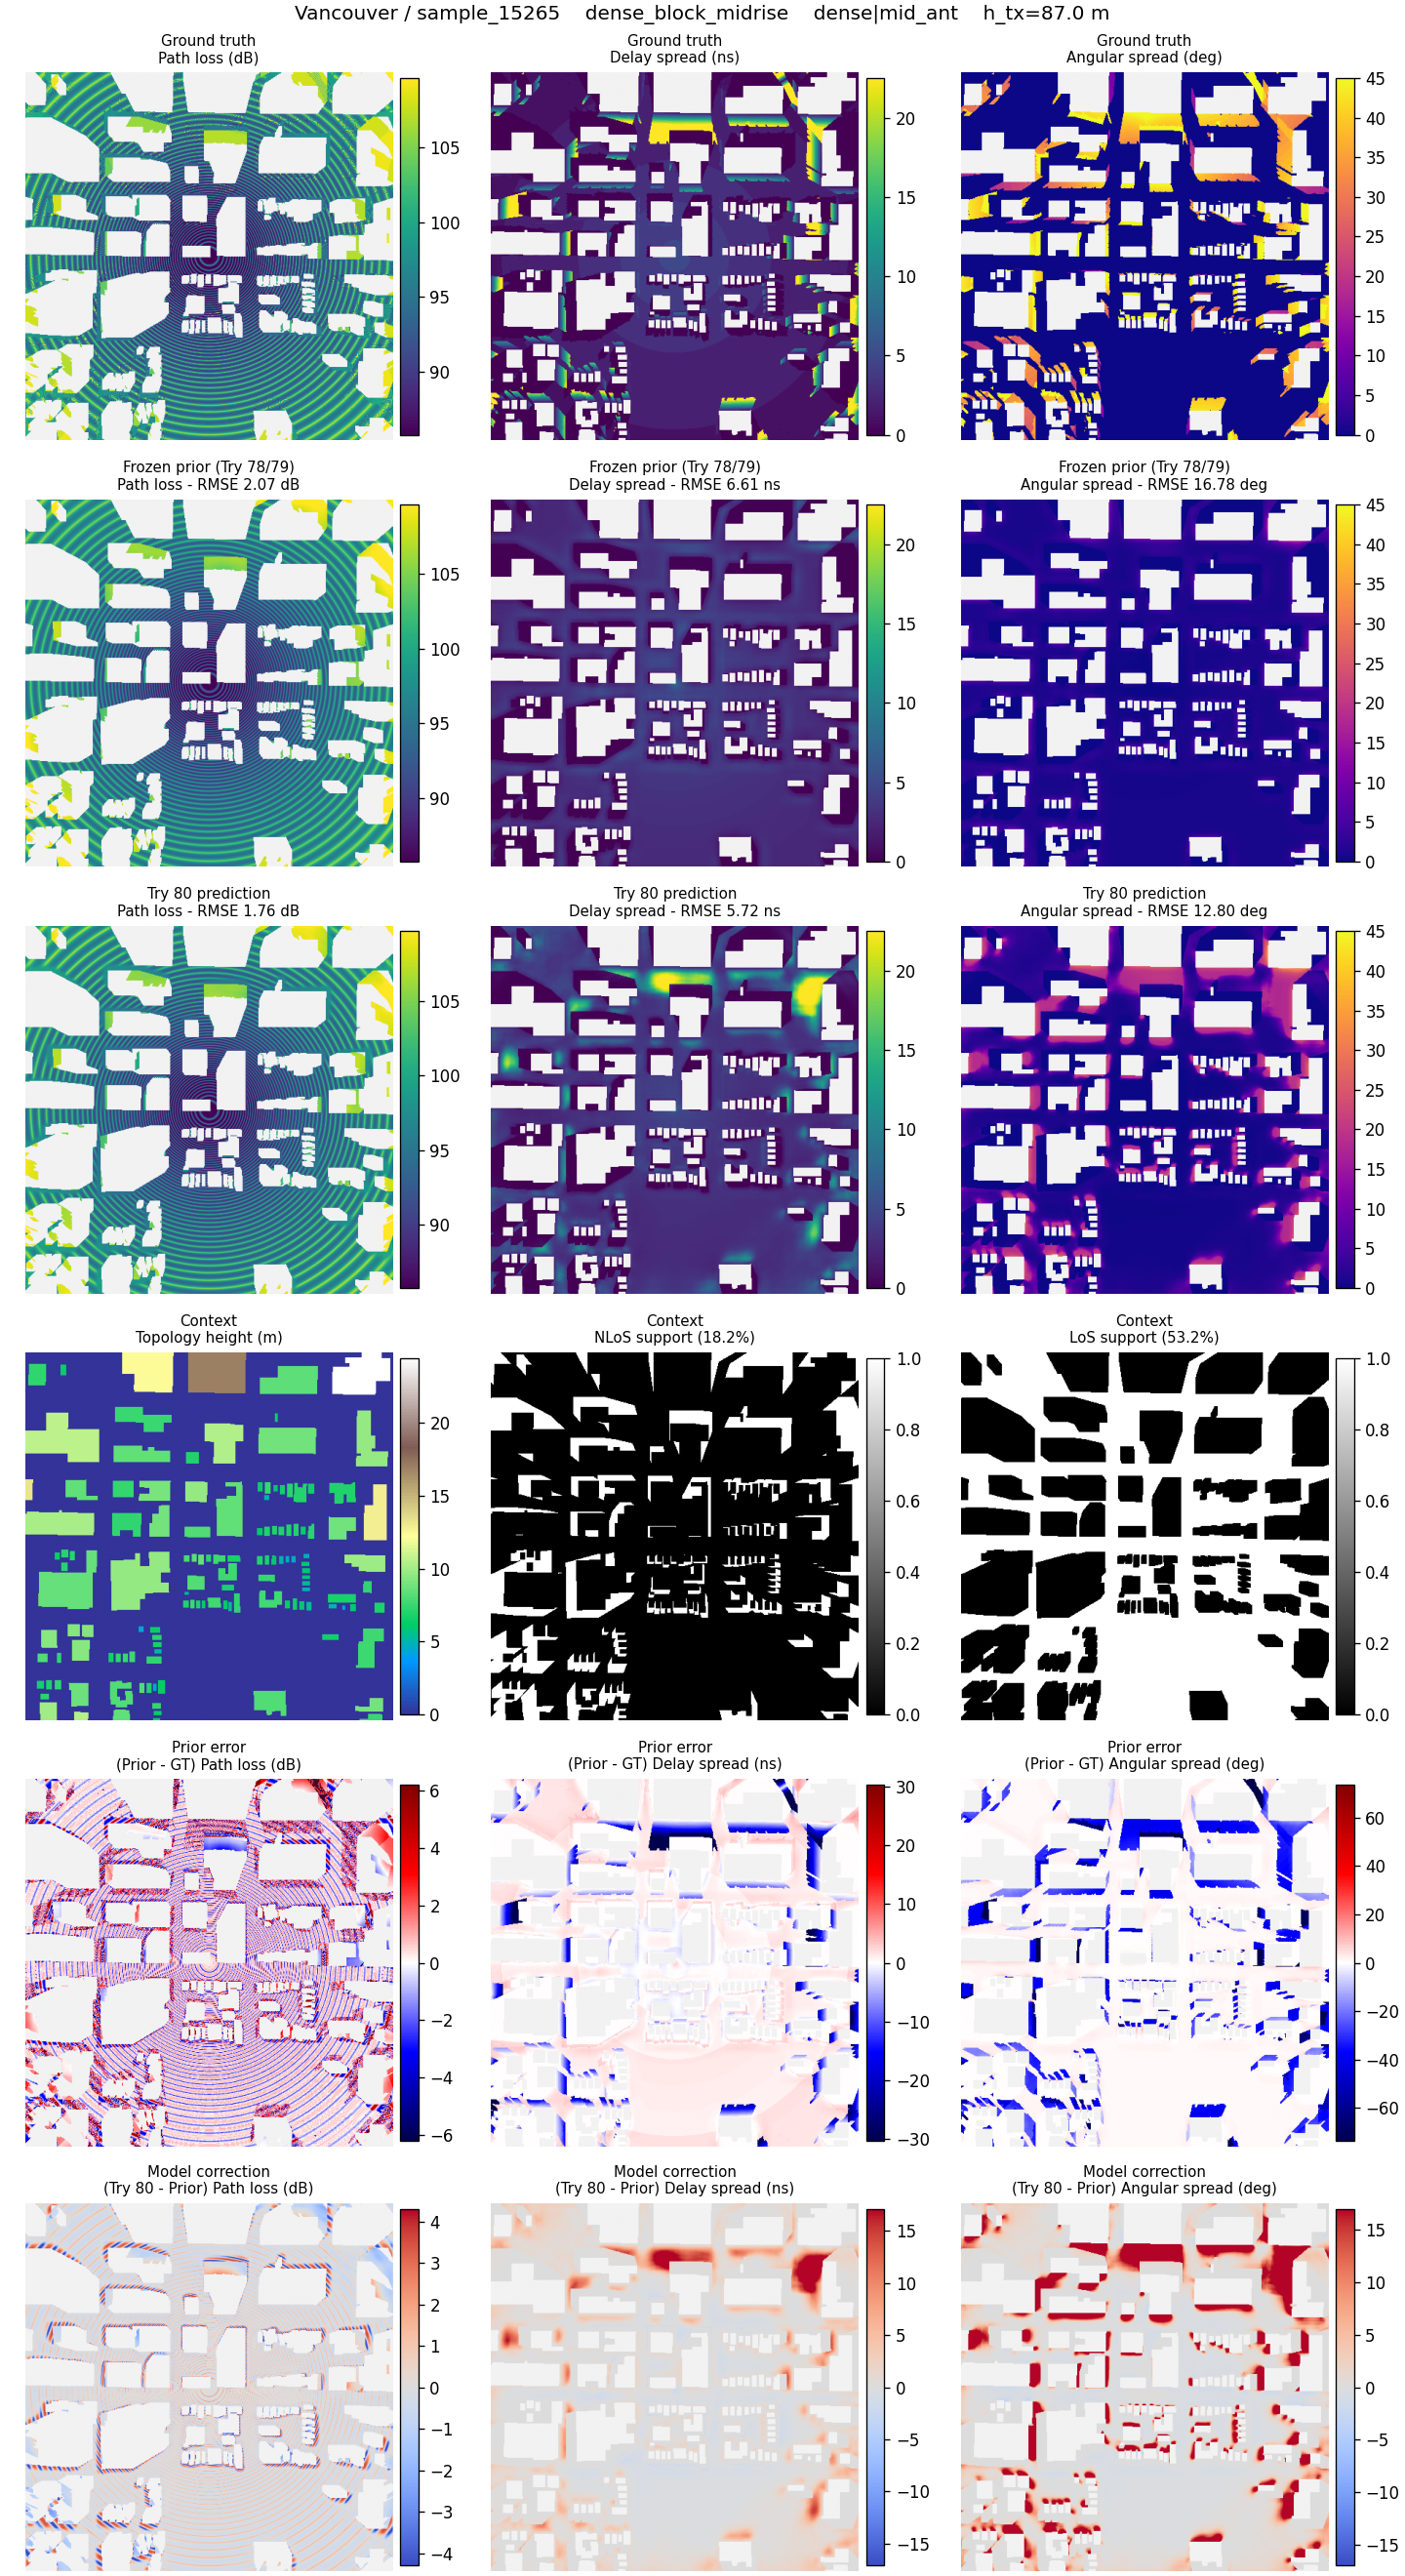
\includegraphics[width=0.82\textwidth,height=0.44\textheight,keepaspectratio]{img/thesis_figures/harpnet_inspection_panels/harpnet_panel_dense_mid_ant_Vancouver_sample_15265_6x3.png}
\caption{Representative final model inspection panel for a dense, mid antenna
held out test sample in Vancouver. Columns are channel attenuation, delay spread, and angular
spread. Rows show ground truth, frozen prior, final prediction,
context/support, prior error, and model residual.}
\label{fig:panel}
\end{figure*}

\subsection{External Metric Context}

Table~\ref{tab:soa} places the final channel attenuation result beside the closest
available path loss side references. The table is deliberately compact and
cautious: datasets, height assumptions, target definitions, and splits differ.
No scalar indoor or link level spread predictor is used as a direct dense map
leaderboard.

\begin{table}[t]
\centering
\caption{Compact comparison with nearby path loss side metrics.}
\label{tab:soa}
\scriptsize
\setlength{\tabcolsep}{3pt}
\begin{tabularx}{\linewidth}{p{0.26\linewidth}p{0.25\linewidth}X}
\toprule
Reference & Attenuation / PL side metric & Reading / caveat \\
\midrule
RadioUNet \cite{radiounet2020} &
\SI{1.6}{dB}--\SI{3.1}{dB} equivalent PL RMSE &
Final attenuation result is in this band; no transmitter height or spread targets. \\
RadioGUNet \cite{radiogunet2025} &
\SI{1.304}{dB} DPM; \SI{1.936}{dB} IRT &
Final attenuation result is between those values; outdoor RadioMapSeer setting. \\
PMNet / ICASSP \cite{pmnet_icassp2023,icassp2023challenge} &
approx.\ \SI{1.38}{dB} converted score &
Final attenuation result is close but higher under a different benchmark setting; scale context only, no joint spread prediction. \\
Gao et al.\ \cite{gao2026} &
\SI{5.59}{dB} ICASSP~2023; \SI{12.19}{dB} ITU~2024 &
Final attenuation result is numerically lower, but this is scale context rather than a
like for like win: recent corridor weighted outdoor PL predictor, no
variable height UAV or joint spread outputs. \\
ReVeal \cite{reveal2025} &
\SI{1.95}{dB} outdoor sparse measurement RMSE &
Final attenuation result is in the same range; sparse mapping rather than dense generation. \\
RMTransformer / PathFinder \cite{rmtransformer2025,pathfinder2025} &
\(\approx\SI{1.82}{dB}\) / \(\approx\SI{1.19}{dB}\) converted references &
Useful scale checks, but random/specialized splits and different assumptions. \\
AIRMap \cite{airmap2025} &
Path gain error \(<\SI{4}{dB}\) against ray tracing &
Same broad digital twin motivation, but path gain and a fixed \(200\times200\) input grid with variable physical extent. \\
\textbf{Final model (ours)} &
\textbf{\SI{1.6947}{dB} attenuation; \SI{26.6882}{ns} DS; \(11.5253^\circ\) AS} &
\textbf{Strict CKM city holdout, centred variable height UAV, dense \(513\times513\) channel attenuation/DS/AS.} \\
\bottomrule
\end{tabularx}
\end{table}

Table~\ref{tab:spread-soa} gives the corresponding spread side context. These
rows are not direct rankings, because the external works report scalar or
link level channel parameters rather than dense CKM maps. They are included so
that the DS/AS results are still positioned against the nearest published
spread prediction literature.

\begin{table*}[t]
\centering
\caption{Spread side comparison with nearby channel parameter prediction work.
External rows give task and metric context, not a direct dense map leaderboard.}
\label{tab:spread-soa}
\scriptsize
\setlength{\tabcolsep}{3pt}
\begin{tabularx}{\textwidth}{p{0.16\textwidth}p{0.35\textwidth}p{0.22\textwidth}X}
\toprule
Reference & Spread side reported output & Relation to this work & Why it is not direct \\
\midrule
Yang et al.\ \cite{yang2019a2gml} &
A2G mmWave delay spread prediction with RF/\(k\)NN; lower RMSE than a lognormal
contrast model. &
Closest early A2G delay spread ML precedent. &
Scalar DS only; no AS, no dense map, no CKM city holdout. \\
Huang et al.\ \cite{huang2025a2gtransformer} &
Transformer UAV predictor; merged data RMSE \SI{4.577}{ns} for RMS DS and
\(1.549^\circ\), \(0.375^\circ\), \(0.864^\circ\), \(0.074^\circ\) for RMS
AAOA, EAOA, AAOD and EAOD. &
Recent UAV mmWave model with delay and angular spread outputs. &
Per link characteristics from coordinates/frequency/location tags, not dense
\(513\times513\) AS/DS maps from topology images. \\
Mi et al.\ \cite{mi2024pointcloud} &
Regression PointNet for indoor \SI{60}{GHz} measurements; predicts RMS DS,
azimuth AS, PL and \(K\)-factor; average AS RMSE \(7.39^\circ\). &
Measurement based DL reference including DS and AS. &
Indoor point cloud task with link level samples, not outdoor UAV CKM generation. \\
Wang et al.\ \cite{wang2023multitasksr} &
Multitask super resolution of path loss, DS, RMS azimuth/elevation AS and
LoS/NLoS maps from lower resolution channel maps. &
Closest map based spread reference reviewed. &
Super resolution starts from a sampled coarse channel map; this paper predicts
dense maps from topology, priors and UAV height with no coarse DS/AS input. \\
\textbf{Final model} &
\textbf{\SI{26.6882}{ns} DS RMSE and \(11.5253^\circ\) AS RMSE.} &
\textbf{Dense channel attenuation/DS/AS maps under the final city holdout setting.} &
\textbf{Should be judged mainly against the frozen spread priors and thesis
targets under the same protocol.} \\
\bottomrule
\end{tabularx}
\end{table*}

The fair conclusion is narrow: the attenuation result is in the same range as
strong dense radio map references, while spread results should be read mainly
against same protocol internal baselines because no external dense topology
conditioned CKM attenuation/DS/AS city holdout benchmark was found. Wang et al.\
are the closest map based spread reference, but their task is channel map super
resolution rather than topology to dense CKM generation.

\subsection{Runtime}

Runtime was measured on Barcelona layouts at full \(513\times513\) resolution
on the same laptop: an AMD Ryzen~5~5600H CPU and an NVIDIA RTX~3050~Ti Laptop
GPU. After checkpoint loading, the generator includes mask generation, frozen
priors, final prediction, and numeric export. It runs in \SI{0.88}{s} per sample
versus \SI{99.89}{s} for the local MATLAB ray tracing path, a \(113.7\times\)
speedup under this setup.

\begin{table}[t]
\centering
\caption{Runtime comparison for one full resolution Barcelona CKM sample on
the same Ryzen~5~5600H / RTX~3050~Ti Laptop hardware.}
\label{tab:runtime}
\scriptsize
\begin{tabularx}{\linewidth}{lXr}
\toprule
Method & Timed path & Time \\
\midrule
MATLAB RT & Pixel receivers outside buildings; attenuation/DS/AS parsed from paths; CPU path &
\SI{99.89}{s} \\
Final generator & Masks, priors, attenuation/DS/AS prediction, numeric export; CUDA mixed precision &
\SI{0.88}{s} \\
\bottomrule
\end{tabularx}
\end{table}

\subsection{Interpretation and Limitations}

The final result supports a hybrid CKM design rather than a claim that one
backbone solves radio mapping in general. The residual model improves a strong
frozen prior on held out validation and test cities, making the gain harder to
dismiss as one easy city mix. The modest delay
spread gain is also informative: after the calibrated prior absorbs the large
geometry trend, remaining spread error is dominated by rare tails, target
quantization, and local blocked/scattered paths.

Limitations remain. The labels come from ray tracing rather than field
measurements, so the result is simulator agreement, not over the air validation.
Target quantization also limits sub unit learning even though the model outputs
continuous channel attenuation, DS, and AS values; the \SI{0.9772}{dB} final
attenuation MAE is already close to the \SI{1}{dB} label step. Finally, the
model is selected under one city holdout split and one final seed, with fixed
frequency, antenna pattern, and simulator assumptions. In particular, every
current scene assumes flat terrain. The reported visibility, distance, and
height relationships therefore do not include terrain-induced blockage or
changes in local ground elevation, and robustness to slopes, valleys, or ridges
has not been demonstrated.

Future work will introduce non-flat digital terrain, express transmitter and
receiver heights relative to local elevation, and recompute visibility,
reflected-path geometry, and morphology features accordingly. Evaluation will
separate relief classes and test whether the frozen priors and residual model
transfer without recalibration. Field measurements remain necessary to
separate simulator fidelity from over-the-air validity. The NLoS calibration
will also remove its current squared raw-prior term $P_0^2$ and refit all
regime weights; the present audit shows large opposing contributions from
$P_0^2$, $P_0$, and the intercept, so this change targets conditioning and
interpretability rather than merely reducing the feature count.

\section{Code Availability}

The reproducibility record is public as source repositories. The standalone CKM
Generator repository contains the interface, command line generator, frozen
calibration files, runtime code, and published checkpoint path
\cite{moreno2026ckmgenerator}. The final training and evaluation repository is
the source record for the paper metrics \cite{moreno2026finalcode}, tied to the
selected \texttt{best\_model.pt} checkpoint and exported breakdown JSON files.
The LaTeX thesis source and project archive are also public
\cite{moreno2026tfgprogress,moreno2026tfgtext}; large data and model artifacts
are external artifacts or Git LFS objects.

\section{Conclusion}

This paper presents a dense variable height UAV CKM surrogate that jointly
predicts channel attenuation, delay spread, and angular spread on unseen cities.
Under strict city holdout, the final model reaches \SI{1.6947}{dB},
\SI{26.6882}{ns}, and \(11.5253^\circ\), respectively. Its main contribution is
a hybrid recipe: fit strong priors on training cities for predictable structure,
then learn bounded residual distributions around those anchors.

The calibrated priors combine coherent two-ray LoS path loss, height dependent
calibration, morphology aware NLoS modelling, visibility switching, and log
domain DS/AS spread statistics. These anchors explain most radial, visibility,
height, and spread scale structure; the residual model improves them by
\SI{0.2436}{dB}, \SI{1.4329}{ns}, and \(2.2909^\circ\) RMSE on the held out
test set. It also improves map correlation from 0.947710 to 0.961055 for
attenuation, from 0.306026 to 0.414692 for delay spread, and from 0.348713 to
0.581783 for angular spread. For the two spread targets this is a relative
MapCorr gain of about \(36\%\) and \(67\%\), respectively, both above the
\(25\%\) mark. This makes clear that the residual model improves map similarity
even when the RMSE reduction is moderate. Continuous transmitter height is
handled through both the priors and a
sinusoidal FiLM path, avoiding per altitude retraining.

The distribution first diagnosis remains the key modelling lesson. NLoS
attenuation residuals are mixture like and prone to mode collapse, while DS/AS
targets are quantized and spike plus tail. GMM style residual heads and
histogram checks prevent visually plausible maps from hiding collapsed
marginals, although rare high spread groups and some false positive spread
patches remain.

For this fixed ray traced CKM setting, \textsc{HARP-Net CKM} is accurate, fast,
and interpretable enough to reduce repeated ray traced map generation, achieving
a measured \(113.7\times\) speedup over the local MATLAB path. The broader
lesson is methodological: diagnose the target distribution, freeze stable
structure in auditable priors, and spend neural capacity on the residual
structure those priors cannot explain. Extending that recipe to non-flat
terrain is the next planned generalization step.

\bibliographystyle{IEEEtran}
\bibliography{TFG}

\end{document}
